\documentclass[10pt]{article}
\usepackage{icmlko}

\icmlmeta{IP 파운데이션 월드모델}{26}{후광인 줄 알았던 것}{팝업 태그의 상관을 편향으로 보고 제거했더니 예측력이 함께 사라졌다 --- 상관은 실체였다}

\begin{document}

\twocolumn[
\icmlheader

\begin{abstract}
노트 25는 게임의 배선 오류를 고쳐 여섯 방향을 모두 살렸고, 나머지 두 도메인에도
같은 오류가 있는지 확인하라고 남겼다. 확인했다. \textbf{아이돌과 게임은 두 공통
축이 서로 다른 인자에 깔끔히 갈리는데}(아이돌: 타깃 폭 PC1 $+$0.81, 굿즈 규모
PC2 $+$0.81) \textbf{팝업은 다섯 축이 전부 PC1에 실린다.} 배선 오류로 보였다.
그런데 팝업 공통 축 둘의 직접 상관은 $+$0.017로 거의 0이다 --- 겹치지 않는다.
그러면 왜 다 같은 인자에 실리는가. 열 축 전체의 상관을 보니 \textbf{평균 $|r|$이
0.210이고 음의 상관이 13\%뿐}이다(무작위면 50\%). 유효 차원도 열 개 축에서
6.37, 다섯 축에서 3.79다. 한 사람이 한 문서를 읽고 열 축을 매기는 데서 오는
후광 효과로 보였다. 제거해 봤다 --- 제1주성분을 잔차화하고 다시 전이했다.
\textbf{팝업이 낀 네 방향이 전부 붕괴했다}(팝업 $\to$ 아이돌 $-$0.0905에서
$-$0.0054로, 게임 $\to$ 팝업 $-$0.0862에서 $+$0.0996으로). 팝업과 무관한 두
방향은 변화가 없다. \textbf{후광 진단이 틀렸다.} 축들의 양의 상관은 평정자
편향이 아니라 실체다 --- 큰 기획은 굿즈도 많고 포토존도 많고 콜라보도 세다.
제1주성분은 잡음이 아니라 ``제작 규모''라는 신호이며, 그것을 빼면 예측할 것이
남지 않는다.
\end{abstract}
]

\section{배선을 확인했다}

노트 25는 게임의 굿즈 규모가 폭 인자에 실려 있던 것을 찾아 고쳤고, 마지막에
이렇게 적었다 --- ``팝업·아이돌의 굿즈 규모가 어느 인자에 실리는지 확인.
같은 오류가 있는지.''

각 도메인의 원자료로 주성분을 뽑고 명명 축이 어디 실리는지 봤다.

\begin{table}[t]
\centering\tsize
\caption{명명 축과 인자의 상관. 굵은 것이 더 강하게 실린 쪽.}
\begin{tabular}{llrr}
\toprule
도메인 & 축 & PC1과 r & PC2와 r \\
\midrule
아이돌 & 타깃 폭 & \textbf{$+$0.81} & $-$0.05 \\
 & 굿즈 규모 & $+$0.21 & \textbf{$+$0.81} \\
\midrule
팝업 & 타깃 폭 & \textbf{$+$0.36} & $-$0.15 \\
 & 굿즈 규모 & \textbf{$+$0.52} & $+$0.03 \\
 & 매장 노출도 & $+$0.34 & $+$0.20 \\
 & 미디어 투입 & $+$0.31 & $+$0.03 \\
 & 입장 허들 & $+$0.06 & $+$0.01 \\
\bottomrule
\end{tabular}
\end{table}

아이돌은 두 공통 축이 서로 다른 인자에 갈린다. 게임도 노트 25의 수정 후 그렇다.
\textbf{팝업만 다섯 축이 전부 PC1에 실린다.}

배선 오류처럼 보였다. 그런데 확인해 보니 팝업의 두 공통 축은 서로 겹치지 않는다.

\begin{table}[t]
\centering\tsize
\caption{공통 축 둘(타깃 폭 $\times$ 굿즈 규모)의 직접 상관.}
\begin{tabular}{lrr}
\toprule
도메인 & n & r \\
\midrule
팝업 & 75 & $+$0.017 \\
아이돌 & 63 & $-$0.144 \\
게임 & 482 & $-$0.128 \\
\bottomrule
\end{tabular}
\end{table}

셋 다 거의 0이다. 팝업의 두 축이 같은 정보를 담고 있는 것이 아니다. 그러면 왜
둘 다 PC1에 실리는가.

\section{후광 효과를 의심했다}

팝업의 열 축 전체를 봤다.

\begin{figure}[t]
\centering
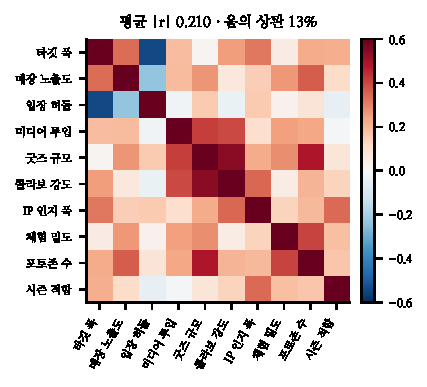
\includegraphics[width=\columnwidth]{figs/heat.pdf}
\caption{팝업 열 축의 상관 행렬. 거의 전부 붉은색(양의 상관)이다.}
\end{figure}

\begin{table}[t]
\centering\tsize
\caption{팝업 사람 태그의 상관 구조(n=75).}
\begin{tabular}{lr}
\toprule
평균 $|r|$ & 0.210 \\
음의 상관 비율 & 13\% \\
\midrule
굿즈 규모 $\times$ 콜라보 강도 & $+$0.543 \\
굿즈 규모 $\times$ 포토존 수 & $+$0.485 \\
미디어 투입 $\times$ 굿즈 규모 & $+$0.415 \\
\bottomrule
\end{tabular}
\end{table}

마흔다섯 쌍 중 서른아홉 쌍이 양의 상관이다. 무작위라면 절반이어야 한다.

\begin{figure}[t]
\centering
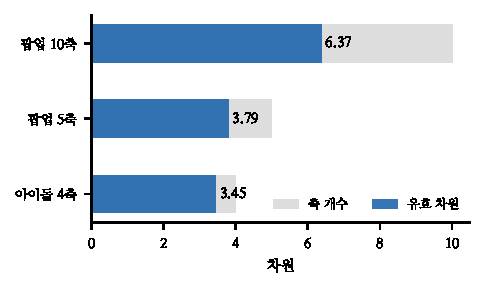
\includegraphics[width=\columnwidth]{figs/dim.pdf}
\caption{유효 차원(참여 비율). 축 개수보다 훨씬 적다.}
\end{figure}

유효 차원도 낮다 --- 열 축에서 6.37, 다섯 축에서 3.79다. 아이돌 네 축은 3.45로
비슷하게 낮다.

한 사람이 한 문서를 읽고 열 축을 연달아 매기면 인상이 전이된다. 심리측정에서
후광 효과라 부르는 것이고, 그렇다면 제1주성분은 평정자 편향이므로 빼는 것이
옳다. 그렇게 가정하고 검정했다.

\section{제거했더니 무너졌다}

팝업 축에서 제1주성분을 잔차화하고 전이를 다시 쟀다.

\begin{figure}[t]
\centering
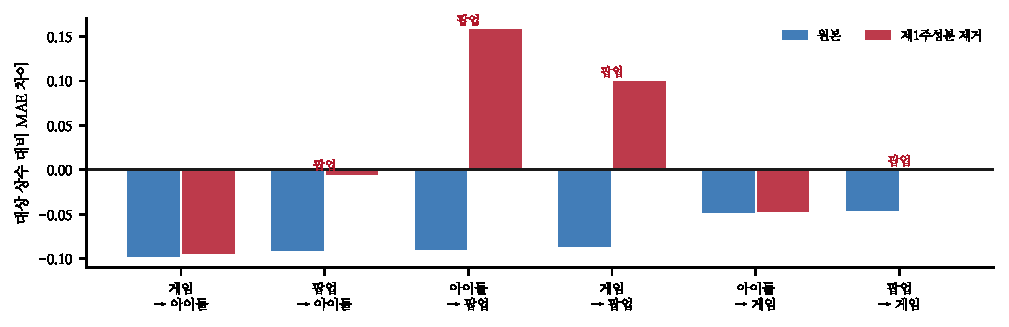
\includegraphics[width=\textwidth]{figs/halo.pdf}
\caption{제1주성분 제거 전후. 팝업이 낀 네 방향만 무너진다.}
\end{figure}

\begin{table}[t]
\centering\tsize
\caption{제1주성분 제거 전후. 순열 2,000회.}
\begin{tabular}{lrrrr}
\toprule
& \multicolumn{2}{c}{원본} & \multicolumn{2}{c}{제거 후} \\
방향 & 차이 & p & 차이 & p \\
\midrule
팝업 $\to$ 아이돌 & $-$0.0905 & 0.001 & $-$0.0054 & 0.407 \\
팝업 $\to$ 게임 & $-$0.0457 & 0.001 & $-$0.0006 & 0.405 \\
아이돌 $\to$ 팝업 & $-$0.0895 & 0.024 & $+$0.1576 & 1.000 \\
게임 $\to$ 팝업 & $-$0.0862 & 0.000 & $+$0.0996 & 1.000 \\
\midrule
아이돌 $\to$ 게임 & $-$0.0476 & 0.002 & $-$0.0473 & 0.002 \\
게임 $\to$ 아이돌 & $-$0.0976 & 0.000 & $-$0.0948 & 0.000 \\
\bottomrule
\end{tabular}
\end{table}

팝업이 낀 네 방향이 전부 유의성을 잃고, 둘은 부호까지 뒤집혀 상수보다 크게
나빠진다. 팝업과 무관한 두 방향은 소수점 넷째 자리까지 그대로다.

\claimx{팝업 태그의 제1주성분은 평정자 편향이 아니라 신호다. 제거하면 팝업이 낀
모든 전이가 무너진다.}{다른 평정자가 독립적으로 매긴 태그에서 같은 상관 구조가
나오면 그것은 개인 편향이 아니라는 추가 증거가 되고, 나오지 않으면 이 결론이
흔들린다.}

\section{왜 상관이 실체인가}

해석은 어렵지 않다. \textbf{큰 기획은 모든 면에서 크다.} 예산이 큰 팝업은 굿즈
종류도 많고, 포토존도 많고, 콜라보 상대도 세고, 홍보도 많이 한다. 축들이 양의
상관을 갖는 것은 평정자가 흐린 것이 아니라 세계가 그렇게 생긴 것이다.

노트 18의 인자 분석이 이미 그렇게 말하고 있었다 --- 팝업 PC1(29\%)에 굿즈
$+$0.42, 포토존 $+$0.40, 콜라보 $+$0.37, 미디어 $+$0.34가 모이고 라벨과 $+$0.319다.
그것을 ``제작 규모''라고 이름 붙였다. 이번에 그것을 후광으로 오인하고 빼려 했던
것이다.

\paragraph{그러면 후광은 전혀 없는가}
알 수 없다. 관측된 상관은 실제 규모 공변과 평정자 편향의 합인데, 이 데이터로는
둘을 분리할 수 없다. 분리하려면 같은 문서를 여러 사람이 독립적으로 매긴 자료가
있어야 한다. \textbf{확실한 것은 관측된 상관의 예측 가치가 크다는 것뿐이다.}

\claimx{축들의 상관을 제거하는 전처리를 하지 않는다. 상관에 담긴 공통 규모 성분이
예측력의 대부분이다.}{평정자 간 자료를 확보해 편향 성분만 골라 뺐을 때 예측력이
유지되거나 오르면, 전체를 빼지 말고 편향만 빼는 것이 옳다.}

\section{두 가지 교훈}

\paragraph{요약 통계의 이상은 진단이 아니다}
``다섯 축이 전부 PC1에 실린다''는 사실 자체는 문제도 정상도 아니다. 노트 25에서는
같은 종류의 관찰(게임 두 축이 둘 다 폭 인자)이 진짜 오류였고, 여기서는 아니었다.
차이는 \emph{그 구조가 예측에 기여하는가}이며, 그것은 빼 보고 재는 수밖에 없다.

\paragraph{독립성은 목표가 아니다}
축을 설계할 때 서로 독립이면 좋겠다고 생각하기 쉽다. 그런데 이 데이터에서는
독립성을 강제하는 순간 예측력이 사라진다. 축은 \emph{서로 다른 것을 재야} 하지
\emph{서로 무관해야} 하는 것이 아니다. 타깃 폭과 굿즈 규모는 상관이 $+$0.017로
독립인데, 그 둘이 함께 실리는 규모 성분이 없으면 둘 다 무력하다.

\section{한계}

\begin{itemize}[leftmargin=1.1em,itemsep=0.15em]
\item 평정자가 한 명이므로 후광 편향과 실제 공변을 분리할 수 없다. ``편향이
      아니다''가 아니라 ``편향이든 아니든 예측에 필요하다''까지만 말할 수 있다.
\item 제거 방식이 제1주성분 잔차화 하나뿐이다. 더 온건한 축소(부분 수축)에서는
      결과가 다를 수 있다.
\item 팝업 n=75에서 뽑은 주성분이라 성분 자체가 불안정하다.
\item 유효 차원 6.37/10은 비교 기준이 없다. 다른 태깅 체계와 견줘야 높고 낮음을
      말할 수 있다.
\end{itemize}

\section{다음}

\begin{enumerate}[leftmargin=1.3em,itemsep=0.15em]
\item 평정자 간 자료 확보 --- 같은 문서를 둘 이상이 독립 태깅. 후광과 실체를 가른다.
\item 부분 수축으로 제거 강도를 조절하며 예측력 곡선 측정.
\item 게임 잔여 난이도($+$0.0289)의 원인 --- 노트 25가 남긴 과제.
\item 네 번째 도메인.
\end{enumerate}

\vspace{0.6em}
\hrule height 0.3pt
\vspace{0.5em}
{\footnotesize
\textbf{참고문헌}\\[0.3em]
Thorndike, E. L. (1920). A constant error in psychological ratings.
\emph{Journal of Applied Psychology}, 4(1), 25--29.\\[0.15em]
Thurstone, L. L. (1947). \emph{Multiple-Factor Analysis}. University of Chicago Press.\\[0.15em]
Cronbach, L. J. (1951). Coefficient alpha and the internal structure of tests.
\emph{Psychometrika}, 16(3), 297--334.\\[0.15em]
Ben-David, S. et al. (2010). A theory of learning from different domains.
\emph{Machine Learning}, 79(1--2), 151--175.
}

\end{document}
